\chapter{الزمن الخاص، وتمدد الزمن، وانكماش الطول}

سنختار كثيرًا وحدات تكون فيها سرعة الضوء $c=1$. في تلك الوحدات يمكن مقارنة سنة من الزمن وسنة ضوئية من المسافة مباشرةً، وتصبح الصيغ أسهل بكثير في القراءة. وكلما كانت $c$ ذات أهمية فيزيائية، أعدنا إدراجها. ويكفي التحليل البعدي لتحديد موضعها.

\section{شبكة الزمكان الغاليلي}

ابدأ بالعلاقة السابقة لأينشتاين بين إطار ساكن وقطار يتحرك بسرعة $v$ على طول محور $x$:
\begin{align}
x' &= x-vt, & t'&=t.
\label{eq:l4-galilean}
\end{align}
تتضمن المعادلة الثانية افتراض نيوتن بوجود زمن كوني. فكل راصد يستخدم شرائح التزامن نفسها، مع أن أصول الإحداثيات المكانية تتحرك بعضها بالنسبة إلى بعض.

افترض أن الراصد في الإطار غير المعلَّم بشرطة يقف بجانب السكة، وأن الراصد في الإطار المعلَّم بشرطة يركب القطار. يحقق أصل القطار $x'=0$، لذا فإن خط عالمه في الإحداثيات غير المعلَّمة بشرطة هو
\begin{equation}
x=vt.
\end{equation}
وذلك الخط المائل هو محور $t'$. وعلى النقيض من ذلك، فإن $t'=t$ تعني أن جميع الخطوط ذات $t'$ الثابت هي الخطوط الأفقية نفسها ذات $t$ الثابت.

\begin{figure}[H]
\centering
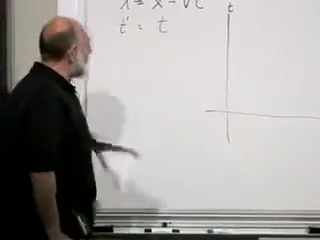
\includegraphics[width=0.72\textwidth]{lecture_04_figure_02.png}
\caption{التحويل الغاليلي وشبكة $t$-$x$ الابتدائية. سيتتبع الأصل المتحرك $x=vt$، بينما يحتفظ الإطاران بخطوط مشتركة للزمن الثابت.}
\lectureframe{00:03:06}
\end{figure}

بحل المعادلة ~\eqref{eq:l4-galilean} بالنسبة إلى الإحداثيات غير المعلَّمة بشرطة نحصل على
\begin{align}
x&=x'+vt'=x'+vt, & t&=t'.
\end{align}
وللمعكوس الصيغة نفسها مع استبدال $v$ بـ $-v$. فإذا كان القطار يتحرك إلى الأمام بالنسبة إلى المحطة، فإن المحطة تتحرك إلى الخلف بالنسبة إلى القطار. وتبقى هذه التبادلية قائمة في النسبية الخاصة، لكن الزمن الكوني لا يبقى.

\section{تصحيح لورنتز}

لا تستطيع التحويلات الغاليليّة أن تجعل سرعة الضوء واحدة في كل إطار قصوري. والعلاقات المصححة هي، أولًا في وحدات $c=1$،
\begin{align}
x'&=\frac{x-vt}{\sqrt{1-v^2}}, &
t'&=\frac{t-vx}{\sqrt{1-v^2}}.
\label{eq:l4-lorentz-natural}
\end{align}
وبإعادة الوحدات المعتادة نحصل على
\begin{align}
x'&=\frac{x-vt}{\sqrt{1-v^2/c^2}}, &
t'&=\frac{t-vx/c^2}{\sqrt{1-v^2/c^2}}.
\label{eq:l4-lorentz-c}
\end{align}

\begin{figure}[H]
\centering
\includegraphics[width=0.74\textwidth]{lecture_04_figure_05.png}
\caption{تحويل لورنتز مع إعادة عوامل $c$.}
\lectureframe{00:09:10}
\end{figure}

عندما يكون $v\ll c$، يكون كل من $v^2/c^2$ و $vx/c^2$ صغيرًا جدًا في الظروف التي تُستخدم فيها الميكانيكا النيوتنية. وعندئذٍ تختزل المعادلة ~\eqref{eq:l4-lorentz-c} إلى النتيجة الغاليليّة. فالنسبية لا تلغي حركيات نيوتن؛ بل تحدد مجال صلاحيتها.

عند $v=c$، ينعدم المقام. ولا يمكن لإطار قصوري أن يتحرك بسرعة الضوء بالنسبة إلى إطار قصوري آخر. ودون ذلك الحد بكثير تكون التصحيحات صغيرة، ولكن بالقرب منه يصبح امتزاج $x$ و $t$ أمرًا لا مفر منه.

اختيرت الحركة على طول $x$، لذا لا تتغير الإحداثيات المستعرضة:
\begin{equation}
y'=y,\qquad z'=z.
\end{equation}
ومن طرائق فهم السبب وضع قضبان مترية مستعرضة متطابقة على القطار وعلى الرصيف. فالراصد الذي يتحرك بسرعة وسطية بين الإطارين يرى القضبان تقترب بسرعات متساوية ومتعاكسة. ولا تتضمن هذه الهيئة أي سمة يمكن أن تجعل أحد القضيبين المستعرضين أقصر من الآخر.

\section{تحويلات لورنتز على امتداد مخروط الضوء}

توجد طريقة هندسية لقراءة المعادلة ~\eqref{eq:l4-lorentz-natural}. اجمع معادلتيها:
\begin{align}
t'+x'
&=\frac{(t-vx)+(x-vt)}{\sqrt{1-v^2}}\\
&=(t+x)\frac{1-v}{\sqrt{1-v^2}}\\
&=(t+x)\sqrt{\frac{1-v}{1+v}}.
\label{eq:l4-null-plus}
\end{align}
واطرح إحداهما من الأخرى بالترتيب المتمم:
\begin{align}
t'-x'
&=\frac{(t-vx)-(x-vt)}{\sqrt{1-v^2}}\\
&=(t-x)\frac{1+v}{\sqrt{1-v^2}}\\
&=(t-x)\sqrt{\frac{1+v}{1-v}}.
\label{eq:l4-null-minus}
\end{align}

\begin{figure}[H]
\centering
\includegraphics[width=0.75\textwidth]{lecture_04_figure_06.png}
\caption{تحويل لورنتز بعد إعادة كتابته بالتركيبين العدميين
$t+x$ و $t-x$. وعاملا المقياس فيهما متبادلان عكسيًا.}
\lectureframe{00:18:45}
\end{figure}

التركيبان $t+x$ و $t-x$ هما إحداثيان على امتداد الاتجاهين الضوئيين عند $45^\circ$. يضغط التحويل الدفعي أحد هذين الاتجاهين ويمد الآخر بالعامل العكسي. وهو لا يدير أيًّا منهما بعيدًا عن $45^\circ$. وهكذا تبقى الأشعة الضوئية أشعةً ضوئية، وهذه هي الصورة الزمكانية لثبات سرعة الضوء.

\begin{classroomqa}
\audiencequestion{يرى الراصد في الإطار المتوسط تجربةً متناظرة، ولكن كيف يثبت ذلك النتيجة لراصدي القطار والرصيف؟
\lecturetimestamp{00:20:48}}
\lecturerresponse{يُستخدم هنا أمر إضافي واحد: إن تلاقي الأحداث ثابت. فإذا التقت أطراف القضبان، كان ذلك التلاقي حدثًا زمكانيًا واحدًا. ويجوز لكل راصد قصوري أن يعيّن له إحداثيات مختلفة، ولكن لا يجوز لأي منهم أن يقسم تلاقيًا واحدًا إلى موضعين مختلفين. والومضات المنبعثة عند التقاء النهايات المتناظرة تجعل هذه الأحداث قابلة للكشف عمليًا. ومن ثم يثبت تناظر الإطار المتوسط وثبات تلاقيي النهايتين أن الأطوال المستعرضة متساوية.}
\end{classroomqa}

\begin{classroomqa}
\audiencequestion{هل يجب أن يكون راكب الدراجة الذي يمثّل الإطار المتوسط موجودًا ماديًا عند منتصف القضبان؟\lecturetimestamp{00:22:25}}
\lecturerresponse{لا. فالإطار المرجعي شبكة كاملة من الراصدين والساعات، لا عينًا واحدة في موضع واحد. وقد يتلقى راكب الدراجة ومضات النهايات لاحقًا ويستدل على مواضع انبعاثها. وما يهم هو الموضع الزمكاني لكل حدث انبعاث، لا الموضع الذي يُستقبل فيه الضوء في نهاية الأمر.}
\end{classroomqa}

إن تركيب السرعات المتعاقبة نتيجة أخرى للتحويل نفسه، لكنه يُترك عمدًا للمحاضرة التالية. أما المهمة الحالية فهي تحديد الكمية الثابتة التي تقيسها ساعة متحركة.

\section{الفاصل الثابت}

في دوران المحاور الديكارتية العادية، تبقى الكمية $x^2+y^2$ دون تغير. وتحفظ تحويلات لورنتز صيغةً تربيعية مختلفة. فمن المعادلة ~\eqref{eq:l4-lorentz-natural}،
\begin{align}
t'^2-x'^2
&=\frac{(t-vx)^2-(x-vt)^2}{1-v^2}\\
&=\frac{t^2-2vtx+v^2x^2-x^2+2vtx-v^2t^2}{1-v^2}\\
&=t^2-x^2.
\label{eq:l4-interval}
\end{align}
تتلاشى الحدود المختلطة، ويحتوي البسط المتبقي على عامل مشترك هو $1-v^2$.

\begin{figure}[H]
\centering
\includegraphics[width=0.76\textwidth]{lecture_04_figure_07.png}
\caption{الاشتقاق على السبورة لـ $t'^2-x'^2=t^2-x^2$.}
\lectureframe{00:33:15}
\end{figure}

مع ثلاثة أبعاد مكانية يكون الثابت هو
\begin{equation}
t'^2-x'^2-y'^2-z'^2=t^2-x^2-y^2-z^2
\end{equation}
في وحدات $c=1$. وعلى نحو أعم، نستخدم فروق الإحداثيات بين حدثين:
\begin{equation}
\Delta s^2
=c^2\Delta t^2-\Delta x^2-\Delta y^2-\Delta z^2.
\label{eq:l4-spacetime-interval}
\end{equation}
ويتفق كل راصد قصوري على هذا العدد، رغم أنهم يختلفون في حدوده المنفصلة للزمان والمكان.

\section{الزمن الخاص والساعات المتحركة}

تخيّل شبكةً من الراصدين الساكنين جرت مزامنة ساعاتهم بتبادل إشارات ضوئية. وتحدد قراءاتهم الزمن الإحداثي $t$. والآن احمل ساعة يد واحدة عبر تلك الشبكة. فقراءتها الخاصة ترافق الساعة على طول خط عالمها؛ وتلك القراءة هي الزمن الخاص.

لحدثين يفصل بينهما فاصل زمني، عرّف
\begin{equation}
c^2\Delta\tau^2
=c^2\Delta t^2-\Delta x^2-\Delta y^2-\Delta z^2.
\label{eq:l4-proper-time}
\end{equation}
وفي بعد مكاني واحد مع $c=1$، يصبح هذا ببساطة
\begin{equation}
\Delta\tau=\sqrt{\Delta t^2-\Delta x^2}.
\end{equation}
ويوازي الجذر التربيعي الصيغة الخاصة بالمسافة العادية، لكن الإشارة السالبة تغيّر الهندسة.

توجد ثلاث حالات:
\begin{align}
\Delta t^2-\Delta x^2 &>0 &&\text{timelike},\\
\Delta t^2-\Delta x^2 &=0 &&\text{lightlike},\\
\Delta t^2-\Delta x^2 &<0 &&\text{spacelike}.
\end{align}
داخل مخروط الضوء يكون الزمن الخاص حقيقيًا. وعلى المخروط، حيث $x=\pm t$، يكون صفرًا رغم أن الحدثين لا يلزم أن يتطابقا. ويمكن لشعاع ضوئي أن يصل بين مثل هذه الأحداث على وجه الدقة. وخارج المخروط يكون الفصل مكانيًا؛ ومن الأفضل وصفه بالمسافة الخاصة الحقيقية $\sqrt{\Delta x^2-\Delta t^2}$ بدلًا من زمن ساعة تخيلي.

\begin{figure}[H]
\centering
\includegraphics[width=0.73\textwidth]{lecture_04_figure_08.png}

\vspace{0.8em}

\begin{tikzpicture}[x=1.0cm,y=1.0cm]
\draw[->] (-3.3,0) -- (3.3,0) node[right] {$x$};
\draw[->] (0,-0.4) -- (0,4.0) node[above] {$t$};
\draw[thick] (0,0) -- (3.0,3.0) node[above right] {$x=t$};
\draw[thick] (0,0) -- (-3.0,3.0) node[above left] {$x=-t$};
\node at (0,2.0) {timelike};
\node at (2.25,1.05) {spacelike};
\node at (-2.25,1.05) {spacelike};
\end{tikzpicture}
\caption{مخروط الضوء على السبورة وتصنيف واضح للفصل الزمني، والضوئي، والمكاني.}
\lectureframe{00:38:40}
\end{figure}

لماذا تساوي المعادلة ~\eqref{eq:l4-proper-time} قراءةَ ساعة؟ بالنسبة إلى ساعة ساكنة، يكون $\Delta x=0$، ومن ثم $\Delta\tau=\Delta t$. وبالنسبة إلى ساعة تتحرك حركة منتظمة، اختر الإطار المعلَّم بشرطة الذي تكون فيه تلك الساعة ساكنة. هناك يكون $\Delta x'=0$، ويعطي الثبات
\begin{equation}
\Delta\tau
=\sqrt{\Delta t'^2-\Delta x'^2}
=\Delta t'.
\end{equation}
ولذلك تعدّ الساعات المتحركة الزمن الخاص.

\begin{classroomqa}
\audiencequestion{هل يُستعمل ``الفاصل بين الحدثين'' و ``قراءة الساعة'' بوصفهما اسمين للشيء نفسه؟
\lecturetimestamp{00:44:49}}
\lecturerresponse{يتطابقان عندما تنتقل ساعة مثالية قصوريًا من أحد الحدثين إلى الآخر. فالفاصل الثابت كمية هندسية؛ أما الفرق بين قراءتي الطرفين للساعة المصاحبة للحركة فهو قياسه الفيزيائي. وعادةً ما تسجل ساعة إحداثية ساكنة فاصلًا مختلفًا للزمن الإحداثي.}
\end{classroomqa}

\section{تمدد الزمن والتزامن}

انظر إلى أصل الإطار المتحرك. يحقق خط عالمه
\begin{equation}
x'=0,\qquad x=vt.
\end{equation}
والخط المائل نفسه هو في آن واحد مسار الساعة المتحركة ومحور $t'$.

\begin{figure}[H]
\centering
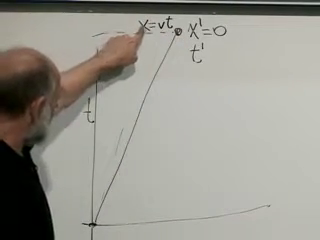
\includegraphics[width=0.72\textwidth]{lecture_04_figure_03.png}
\caption{الأصل المتحرك: $x=vt$، و$x'=0$، ومحور $t'$ هي ثلاثة أوصاف لخط العالم نفسه.}
\lectureframe{00:48:18}
\end{figure}

طبّق الفاصل الثابت بين الأصل المشترك ونقطة لاحقة على ذلك الخط العالمي:
\begin{align}
t'^2-x'^2&=t^2-x^2,\\
t'^2&=t^2-v^2t^2,\\
t'&=t\sqrt{1-v^2}.
\label{eq:l4-time-dilation-natural}
\end{align}
ومع إعادة $c$ نحصل على
\begin{equation}
\Delta\tau=\Delta t\sqrt{1-\frac{v^2}{c^2}}
=\frac{\Delta t}{\gamma},
\qquad
\gamma=\frac{1}{\sqrt{1-v^2/c^2}}.
\label{eq:l4-time-dilation}
\end{equation}

\begin{figure}[H]
\centering
\includegraphics[width=0.73\textwidth]{lecture_04_figure_09.png}
\caption{نتيجة تمدد الزمن على السبورة: يتراكم على الساعة المتحركة $t'=t\sqrt{1-v^2}$ في وحدات يكون فيها $c=1$.}
\lectureframe{00:50:45}
\end{figure}

يقول الراصد الساكن إن الساعة المتحركة تسير ببطء. وتقتضي المعاملة بالمثل أن يقول الراصد المتحرك الشيء نفسه عن الساعات الساكنة. ولا يوجد تناقض، لأن الوصفين يقارنان زوجين مختلفين من الأحداث المتباعدة.

في الواقع، إذا كانت قيمة $t'$ ثابتة في المعادلة ~\eqref{eq:l4-lorentz-natural}، فإن ذلك يقتضي
\begin{equation}
t-vx=\text{constant}.
\label{eq:l4-simultaneity}
\end{equation}
خطوط التزامن لدى الراصد المتحرك مائلة بالنسبة إلى الخطوط الأفقية $t=\text{constant}$. ويعدّ كل راصد مجموعة مختلفة من قراءات الساعات المتباعدة متزامنة. ومتى أُبقي هذا الاختلاف ظاهرًا، اتسق التباطؤ المتبادل للساعات.

\begin{figure}[H]
\centering
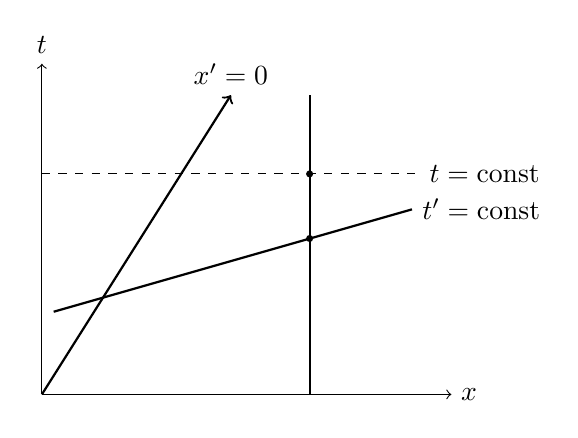
\begin{tikzpicture}[x=1cm,y=1cm]
\draw[->] (0,0) -- (0,4.2) node[above] {$t$};
\draw[->] (0,0) -- (5.2,0) node[right] {$x$};
\draw[thick,->] (0,0) -- (2.4,3.8) node[above] {$x'=0$};
\draw[dashed] (0,2.8) -- (4.8,2.8)
  node[right] {$t=\mathrm{const}$};
\draw[thick] (0.15,1.05) -- (4.7,2.35)
  node[right] {$t'=\mathrm{const}$};
\draw[thick] (3.4,0) -- (3.4,3.8);
\fill (3.4,2.8) circle (0.045);
\fill (3.4,1.98) circle (0.045);
\end{tikzpicture}
\caption{يقارن تمدد الزمن المتبادل قراءات الساعات على شرائح تزامن مختلفة.}
\end{figure}

\section{مسارا التوأمين}

يبدأ توأمان من الحدث نفسه. يبقى أحدهما عند $x=0$. ويسافر الآخر مبتعدًا بسرعة $v$، ثم يعكس اتجاهه ويعود بالسرعة نفسها. وعندما يلتقيان من جديد يقارنان كل عملية فيزيائية يمكن أن تصلح ساعةً: ساعات اليد، وخفقات القلب، والأيض، أو حتى الشيخوخة نفسها.

لنفترض أن كل نصف من الرحلة يستغرق زمنًا إحداثيًا مقداره $T$ في إطار التوأم المقيم. يكون الزمن الخاص للتوأم المقيم
\begin{equation}
\tau_{\mathrm{home}}=2T.
\end{equation}
وإحداثيا حدث الانعطاف هما $(vT,T)$. ولذلك تسهم المرحلة الأولى من الرحلة بمقدار
\begin{align}
\tau_{\mathrm{leg}}
&=\sqrt{T^2-v^2T^2}
=T\sqrt{1-v^2}.
\end{align}
وتسهم مرحلة الإياب بالمقدار نفسه، ومن ثم
\begin{equation}
\tau_{\mathrm{travel}}=2T\sqrt{1-v^2}<2T.
\label{eq:l4-twin}
\end{equation}

\begin{figure}[H]
\centering
\includegraphics[width=0.73\textwidth]{lecture_04_figure_10.png}

\vspace{0.8em}

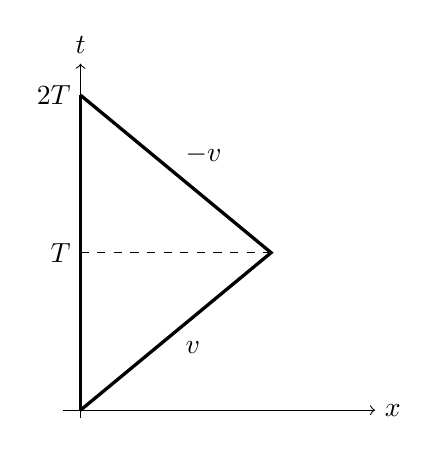
\begin{tikzpicture}[x=1.1cm,y=1cm]
\draw[->] (-0.2,0) -- (3.4,0) node[right] {$x$};
\draw[->] (0,-0.1) -- (0,4.4) node[above] {$t$};
\draw[very thick] (0,0) -- (0,4);
\draw[very thick] (0,0) -- (2.2,2) -- (0,4);
\draw[dashed] (0,2) -- (2.2,2);
\node[left] at (0,2) {$T$};
\node[left] at (0,4) {$2T$};
\node[below right] at (1.1,1.0) {$v$};
\node[above right] at (1.1,3.0) {$-v$};
\end{tikzpicture}
\caption{خط العالم للتوأم المقيم ومرحلتا الرحلة. أزمنتها الخاصة مختلفة لأنها مسارات مختلفة عبر الزمكان.}
\lectureframe{00:59:35}
\end{figure}

لا يوجد تناقض في عدم تساوي العمرين. فمسار الرحلة يتضمن انعطافًا، ولا يرتبط بالمسار المستقيم للتوأم المقيم بتناظر واحد لإطار قصوري. وفي الهندسة الإقليدية العادية يكون أيضًا للمسار المستقيم والمسار المنكسر بين نقطتين طولان مختلفان. وتعكس هندسة مينكوفسكي أيَّ المسارين له الفاصل الأكبر، لكن المقارنة تظل هندسية.

\section{التسارع والساعة المثالية}

\begin{classroomqa}
\audiencequestion{عند الانعطاف تكون الفيزياء مختلفة ويتسارع المسافر. فهل يُبطل ذلك حساب الساعة؟
\lecturetimestamp{01:02:19}}
\lecturerresponse{التسارع حقيقي ويساعد على تحديد عدم التناظر؛ ولا ينبغي محاولة التخلص منه بالمجادلة. والزاوية الحادة ليست إلا تمثيلًا مثاليًا، ويمكن استبدالها بانعطاف ذي مدة منتهية. والافتراض الفيزيائي الإضافي هو أن الساعة، إذا كانت صغيرة بما يكفي ومحكمة الصنع، تكون غير حساسة لتسارع معتدل وتستمر في تسجيل الزمن الخاص. وقد تتشوه ساعة كبيرة أو هشة أو تنكسر، لكن ذلك عيب في الآلية لا في الفاصل الزمكاني.}
\end{classroomqa}

هذا الافتراض الخاص بالساعة المثالية لا يُستمد من تحويل لورنتز وحده. بل يُختبَر من خلال سلوك آليات الساعات الفعلية. وتُعد الذرة تقريبًا أفضل بكثير من ساعة يبلغ عرضها مئات الأميال، لأن الآلية المدمجة أشد مقاومة للتشوه تحت تأثير التسارع أو الجاذبية. وإن استحضار النسبية العامة بالاسم لن يزيل هذه المسألة الفيزيائية؛ إذ سيظل لا بد من معرفة كيف تستجيب الآلية المختارة لبيئتها.

\begin{classroomqa}
\audiencequestion{هل يمكن تجزئة مسار متسارع إلى فترات قصيرة يبقى فيها التحليل القصوري صالحًا؟\lecturetimestamp{01:09:08}}
\lecturerresponse{نعم. قسِّم المنحنى إلى مقاطع قصيرة تكاد تكون مستقيمة، واحسب الزمن الخاص على كل مقطع، ثم اجمع النتائج. وهذا هو النظير الزمكاني لإيجاد طول منحنى عادي من كثير من القطع المستقيمة الصغيرة. وفي حد المتصل،
\[
\tau=\int \sqrt{1-\frac{v(t)^2}{c^2}}\,dt,
\]
وذلك لحركة في زمكان مستوٍ موصوفة في نظام إحداثيات قصوري.}
\end{classroomqa}

\section{ما يراه التوأمان}

يمكن جعل القراءات النهائية للساعتين إجرائيةً بإرسال نبضات ضوئية. علِّم فواصل مقدار كل منها ثانية واحدة من الزمن الخاص على خطي العالم كليهما، ودَع كل توأم يطلق نبضة عند كل علامة. أثناء مرحلة الابتعاد، تصل النبضات الواردة من التوأم الآخر متباعدة. وأثناء العودة، تصل متقاربة. وهذا هو تأثير دوبلر النسبي معبَّرًا عنه مباشرةً على مخطط الزمكان.

\begin{figure}[H]
\centering
\includegraphics[width=0.73\textwidth]{lecture_04_figure_11.png}
\caption{الإشارات الضوئية المتبادلة بين خط العالم للمقيم وخط العالم للمسافر. فالتباعد في وصولها في مرحلة الابتعاد والتقارب في وصولها في مرحلة العودة يفسران جميع النبضات المنبعثة.}
\lectureframe{01:12:55}
\end{figure}

لا يختفي أي إطار مرجعي في هذا الوصف. فكل راصد يتلقى في نهاية المطاف جميع النبضات التي يبعثها الآخر، لكن معدلات استقبالها تعتمد على الحركة النسبية. والانزياح الأحمر في مرحلة الابتعاد والانزياح الأزرق في مرحلة العودة ليسا تأثيرين متساويي المدة على المسارين، لذا فإن عدَّ جميع النبضات المستقبلة يتفق مع مقارنة الزمن الخاص.

\begin{classroomqa}
\audiencequestion{إذا كان المسافر العائد يستقبل ضوءًا منزاحًا نحو الأزرق، أفيمكنه أن يتلقى طاقةً أكثر مما أصدره المصدر؟
\lecturetimestamp{01:13:50}}
\lecturerresponse{يتطلب ذلك السؤال تعريف الطاقة في النسبية واعتمادها على الإطار المرجعي، وهو ما لم نطوره بعد. وهذا سؤال معقول، لكن الإحداثيات وعدَّ النبضات وحدهما لا يكفيان لتسوية حسابات الطاقة، ولا سيما بالنسبة إلى راصد متسارع. لذلك ينبغي تأجيل الجواب بدلًا من تخمينه.}
\end{classroomqa}

\section{اتجاه مكاني مضغوط}

\begin{classroomqa}
\audiencequestion{افترض أن أحد الاتجاهات المكانية مضغوط. هل يمكن لأحد التوأمين أن يتحرك بانتظام على امتداده، ويعود إلى موضع البداية، ويتجنب التسارع تمامًا؟ فما الذي يميز التوأمين إذن؟\lecturetimestamp{01:15:14}}
\lecturerresponse{ينبغي أن يُتخيل الفضاء من داخله على أنه أسطوانة، لا صفيحة منحنية داخل فضاء أكبر؛ فلا حاجة إلى أي تسارع شعاعي. ومع ذلك، يواجه الراصد العائد الخاصية العالمية المتمثلة في أن الأمكنة نفسها تتكرر. وهذا يدل على لاتناظر، لكن الجواب الكامل يتطلب معالجة دقيقة للنسبية الخاصة مع التطابق المكاني. ويُترك السؤال هنا مفتوحًا بدلًا من الإجابة عنه ارتجالًا.}
\end{classroomqa}

\begin{figure}[H]
\centering
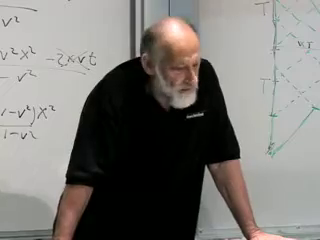
\includegraphics[width=0.72\textwidth]{lecture_04_figure_04.png}

\vspace{0.8em}

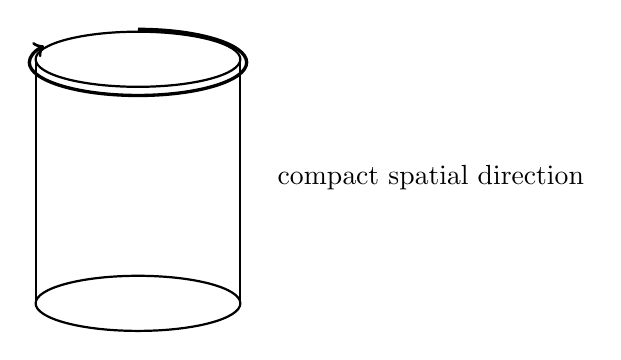
\begin{tikzpicture}[x=1cm,y=1cm]
\draw[thick] (0,0) ellipse (1.3 and 0.35);
\draw[thick] (-1.3,0) -- (-1.3,-3.1);
\draw[thick] (1.3,0) -- (1.3,-3.1);
\draw[thick] (0,-3.1) ellipse (1.3 and 0.35);
\draw[->,very thick] (0.0,0.38) arc (90:-210:1.38 and 0.42);
\node[right] at (1.65,-1.5) {compact spatial direction};
\end{tikzpicture}
\caption{مسألة الفضاء المضغوط كما رُسمت على اللوح، مع تمثيل أسطواني جوهري واضح. وهي مسألة تتعلق بالتطابق العالمي، لا بحركة حول أسطوانة مُضمَّنة في بُعد شعاعي إضافي.}
\lectureframe{01:17:56}
\end{figure}

\section{يُقاس الطول على مقطع تزامن}

في مسألة من مسائل النسبية الخاصة، ارسم أولًا مخطط الزمكان. خذ قضيبًا متريًا ساكنًا في الإطار غير المعلَّم بشرطة، وطرفاه عند $x=0$ و$x=1$. ومع مرور الزمن، يرسم الطرفان خطَّي عالم رأسيين. ويكنس القضيب شريطًا بينهما.

يجب على الراصد المتحرك أن يقيس كلا الطرفين عند قيمة واحدة من زمن الإطار المتحرك $t'$. ومن المعادلة ~\eqref{eq:l4-simultaneity}، فإن المقطع المار بالمبدأ الذي فيه $t'=0$ يحقق
\begin{equation}
t=vx
\end{equation}
بوحدات $c=1$. وهو يقطع الطرف الأيمن $x=1$ عند $t=v$.

\begin{figure}[H]
\centering
\includegraphics[width=0.73\textwidth]{lecture_04_figure_12.png}

\vspace{0.8em}

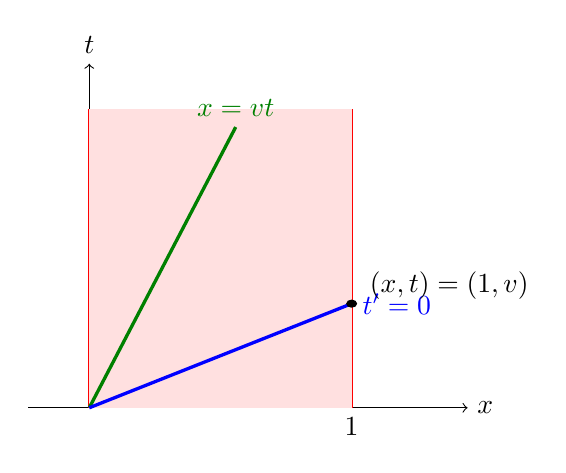
\begin{tikzpicture}[x=1.55cm,y=1.15cm]
\draw[->] (-0.5,0) -- (3.1,0) node[right] {$x$};
\draw[->] (0,0) -- (0,3.8) node[above] {$t$};
\draw[very thick,red] (0,0) -- (0,3.3);
\draw[very thick,red] (2.15,0) -- (2.15,3.3);
\fill[red!12] (0,0) rectangle (2.15,3.3);
\draw[very thick,green!50!black] (0,0) -- (1.2,3.1)
  node[above] {$x=vt$};
\draw[very thick,blue] (0,0) -- (2.15,1.15)
  node[right] {$t'=0$};
\fill (2.15,1.15) circle (0.045);
\node[right] at (2.22,1.35) {$(x,t)=(1,v)$};
\node[below] at (2.15,0) {$1$};
\end{tikzpicture}
\caption{يقوم قضيب ساكن بكنس شريط زمكاني. والطول الذي يقيسه الراصد المتحرك هو المسافة بين طرفيه على مقطع واحد من $t'=\mathrm{const}$.}
\lectureframe{01:24:20}
\end{figure}

الفاصل المختار بين الطرفين شبيه بالمكان، لذا نستخدم الصيغة المكانية الموجبة للمقدار الثابت:
\begin{equation}
x'^2-t'^2=x^2-t^2.
\end{equation}
وعند الطرف المختار، $t'=0$ و$x=1$ و$t=v$. ومن ثم
\begin{align}
x'^2&=1-v^2,\\
x'&=\sqrt{1-v^2}.
\end{align}
إذًا يُقاس طول السكون $L$ في الإطار المتحرك على أنه
\begin{equation}
L'=L\sqrt{1-v^2/c^2}=\frac{L}{\gamma}.
\label{eq:l4-length-contraction}
\end{equation}

\begin{figure}[H]
\centering
\includegraphics[width=0.76\textwidth]{lecture_04_figure_13.png}
\caption{البناء الهندسي المكتمل لانكماش الطول، والنتيجة على اللوح $x'=\sqrt{1-v^2}$ لطول سكوني مقداره وحدة واحدة.}
\lectureframe{01:28:10}
\end{figure}

والعبارة العكسية صحيحة أيضًا: إذ ينسب راصد الرصيف طولًا أقصر إلى القضيب المتري الطولي للقطار. ومرة أخرى، يختار الراصدان حدثين طرفيين متزامنين مختلفين، لذا فالتبادلية ليست متناقضة.

\section{أسئلة في النهاية}

\begin{classroomqa}
\audiencequestion{هل ينتشر شيء غير الضوء بسرعة الضوء؟ وعلى وجه الخصوص، ماذا عن الجاذبية؟\lecturetimestamp{01:29:29}}
\lecturerresponse{تتنبأ النسبية العامة بموجات ثقالية تنتشر بسرعة $c$. وفي وقت هذه المحاضرة، كانت الأدلة تأتي على نحو غير مباشر من أنظمة مثل النجوم النابضة الثنائية؛ ولم تكن الموجات الثقالية قد كُشفت مباشرة بعد.\editorialnote{تغيّر الوضع التجريبي بعد هذه المحاضرة في 2006. فقد رصد LIGO مباشرة GW150914 في 2015، وأظهر الرصد المشترك لـ GW170817 ونظيره الكهرومغناطيسي في 2017 أن سرعتي انتشار الجاذبية والضوء تتفقان ضمن بضع أجزاء في $10^{15}$. انظر \url{https://ligo.org/detections/gw150914/} و\url{https://doi.org/10.1103/PhysRevLett.119.251302}.}}
\end{classroomqa}

\begin{classroomqa}
\audiencequestion{هل يستطيع رائد فضاء أن يقطع مسافة مقدارها سنوات ضوئية كثيرة في زمن خاص أقل من قيمة تلك المسافة عندما تُعبَّر بالسنوات الضوئية؟ وهل يعني ذلك أنه يتحرك أسرع من الضوء؟\lecturetimestamp{01:30:38}}
\lecturerresponse{زمن رائد الفضاء الخاص هو $\sqrt{\Delta t^2-\Delta x^2}$، وهو أصغر من الزمن الإحداثي $\Delta t$. وفي الإطار القصوري لرائد الفضاء، تكون المسافة بين النجمين منكمشة وفق لورنتز. ويتحرك النجمان بسرعة $-v$، لا أسرع من الضوء؛ فثمة ببساطة مسافة منكمشة أقل لقطعها.}
\end{classroomqa}

إذا بدأ رائد الفضاء من السكون ثم تسارع، فإن الوصف يتبدل عبر تعاقب من الأطر القصورية اللحظية. ويمكن أن تتغير المسافة المحسوبة إلى النجوم خلال ذلك الانتقال. ولا يمكن تطبيق تحويل لورنتز ثابت واحد على التاريخ المتسارع بأكمله، لكن الزمن الخاص الكلي يظل يُحسب بجمع المساهمات على طول خط العالم. وينطبق القول نفسه على توأم واقعي ينطلق، وينعطف، ويتباطأ، بدلًا من أن يولد وهو يسير بسرعة الرحلة.

\begin{classroomqa}
\audiencequestion{هل تنشأ هذه الألغاز من معاملة الزمن على أنه مميز؟ وهل يجب أن نسميه بُعدًا رابعًا؟\lecturetimestamp{01:36:43}}
\lecturerresponse{ليس من الضروري أن نبدأ بالشعار القائل إن الزمن بُعد رابع. فتحويل لورنتز نفسه يفرض تداخل المكان والزمان، بينما يعامل الفاصل $t^2-x^2-y^2-z^2$ كليهما بوصفهما جزأين من هندسة واحدة، مع اختلاف الإشارة بين الزمان والمكان. عند السرعات المنخفضة يصبح هذا التداخل مهمَلًا، وتعود الحدوس النيوتونية المألوفة. أما عند السرعات النسبية، فلا يمكن النظر إلى المكان والزمان على أنهما منفصلان انفصالًا جوهريًا.}
\end{classroomqa}

لذلك فإن تمدد الزمن، وانكماش الطول، ومقارنة التوأمين، واختصار زمن الرحلة، ليست حيلًا منفصلة. فهي جميعًا تتبع من ثلاث عادات: تحديد الأحداث الجاري مقارنتها، ورسم هندستها في الزمكان، واستخدام الفاصل الثابت.